% Add "answers" option to print the answers
%\documentclass[addpoints,answers]{exam}
\documentclass[addpoints]{exam}

\usepackage[utf8]{inputenc}
\usepackage{calc}
\usepackage{listings}
\usepackage{xcolor}
\usepackage{xspace}

\definecolor{codegreen}{rgb}{0,0.6,0}
\definecolor{codegray}{rgb}{0.5,0.5,0.5}
\definecolor{codepurple}{rgb}{0.58,0,0.82}

\lstdefinestyle{Cstyle}{
    commentstyle=\color{codegreen},
    keywordstyle=\color{magenta},
    numberstyle=\tiny\color{codegray},
    stringstyle=\color{codepurple},
    basicstyle=\ttfamily\small,
    breakatwhitespace=true,         
    breaklines=true,                 
    captionpos=b,                    
    keepspaces=true,                 
    numbers=left,                    
    numbersep=5pt,                  
    showspaces=false,                
    showstringspaces=false,
    showtabs=false,                  
    tabsize=4
}

\lstset{style=Cstyle}

% \makebox[\textwidth]{Name:\enspace\hrulefill}
%  
% \vspace{5mm}
%\makebox[\textwidth]{Instructor’s name:\enspace\hrulefill}

\newcommand{\truefalse}
{		\begin{checkboxes}
			 \choice True
			 \choice False. Explanation: 
		\end{checkboxes}
		\vspace{10pt}
}

\newcommand{\answerspace}[1]
{
	\ifprintanswers
	\else
		\setlength{\mylength}{10pt}%
		%\noindent\rule{\mylength}{20pt}
		%\vspace{\fpeval{1.2*(#1)}}
		\vspace{#1\mylength}
	\fi
}
\newlength{\mylength}

\newcommand\pf[1]{\textcolor{red}{PF: #1}}
\newcommand\am[1]{\textcolor{blue}{AM: #1}}

\newcommand{\answer}[1]{\begin{solution}{#1}\end{solution}}
\newcommand{\ra}{$\rightarrow$\xspace}



%\usepackage{listings}
\usepackage{color}
\usepackage{lastpage}
\usepackage{verbatim}
\usepackage{fancyvrb}
\usepackage{graphicx}
\usepackage{float}
\usepackage{algorithm}
\usepackage{algpseudocode}
\usepackage{minted}

%\pagestyle{fancy}
%\fancyfoot[C]{{\thepage} of \pageref{LastPage}}
\RecustomVerbatimCommand{\VerbatimInput}{VerbatimInput}{}

\renewcommand{\solutiontitle}{\noindent\textbf{Solution sketch: }}
\renewcommand{\pf}[1]{}

\newcommand{\boxedanswer}[2]{\ifprintanswers\answer{#2}\else\makeemptybox{#1}\fi}

\definecolor{SolutionColor}{rgb}{0.8,0.9,1}


\cfoot{Page \thepage\ of \pageref{LastPage}}

\rhead{Initials: \rule{20mm}{0.4pt}}



%%%%%%%%%%%%%%%%%%%%%%%%%%%%%%%%%%%%%%%%
\begin{document}
\fvset{numbers=left,numbersep=3pt}
\thispagestyle{empty}

\begin{center}
  {\LARGE CS 408 Fall 2026 -- Homework 2\\}

  {\Large Deadline: Friday, September 25th \textbf{at 6p} \\}

  \vspace{20mm}
  \fbox{
    \fbox{\parbox{5.5in}{\centering
        \begin{itemize}
        \item The homework is open notes, open book.
        \item Please upload an annotated version of this pdf, ensuring
          that each answer fits in the box following each
          question.
        \item All solutions must be \textbf{handwritten}; typed
          work will not receive any credit. You may annotate the pdf
          directly, no need to print out and rescan.
        \item No AI tools allowed.
        \item No collaboration with your peers of any kind allowed on
          this homework.
        \item Homeworks are due at \textbf{6PM}. Anything submitted
          after \textbf{6PM} will not be accepted.
        \item Provide complete and clear but concise answers. Clearly
          explain your answers where required.
	\end{itemize}
      }}}
\end{center}

\vspace{13mm}
\begin{center}
	\makebox[0.6\textwidth]{
		\combinedgradetable[h][questions]
	}
\end{center}
%\begin{center}\combinedgradetable[h][questions]\end{center}
\vspace{28mm}

\begin{center}
\makebox[\textwidth]{\textbf{Name (please print)}: \rule{100mm}{0.8pt} }
\end{center}

\newpage
\begin{questions}

\question Consider the following CFG. \\
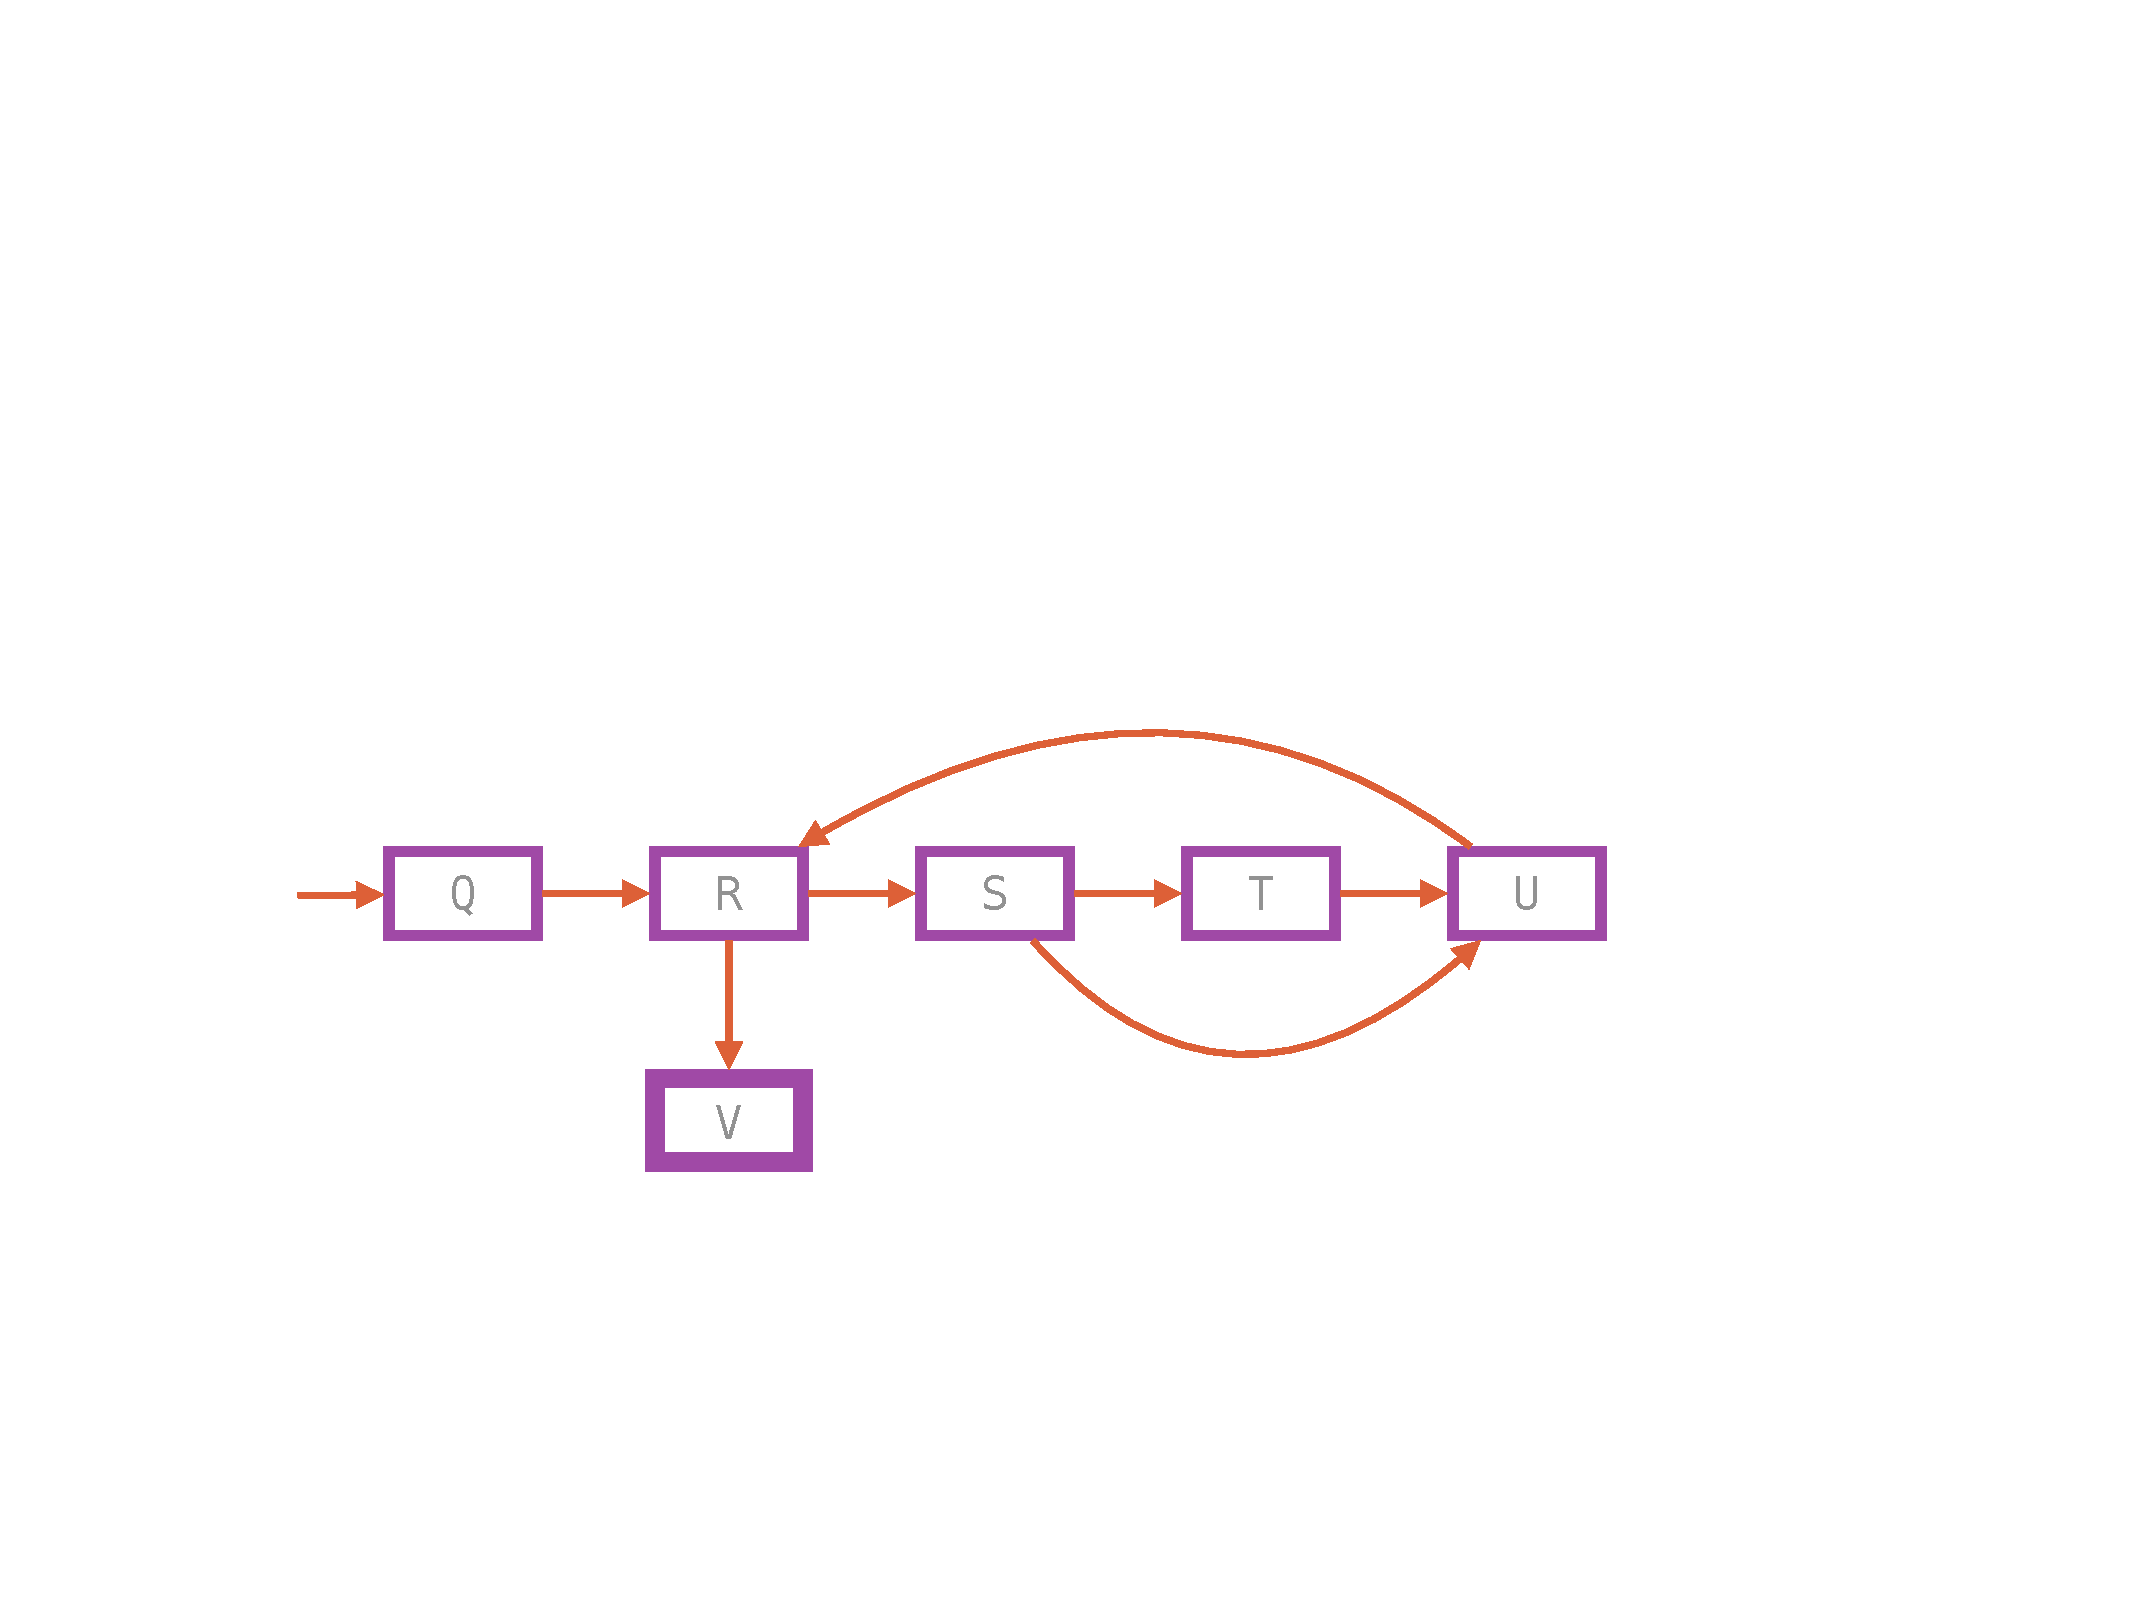
\includegraphics[width=0.8\textwidth]{figs/CFG-1.pdf}

\begin{parts}
\part[8] Provide a simple example of a python function that generates
  this control-flow graph. It should be possible for a test set to
  achieve both 100\% node coverage and 100\% edge coverage on your
  program. Do not define any auxiliary functions, unless absolutely
  necessary. Label the source code statements with comments
  corresponding to the CFG node names. %
  \boxedanswer{5in}{ %
    FILL IN HERE.  }
\newpage
\part[1] How many test requirements are needed by node coverage?
  \boxedanswer{1.5in}{ %
  }

\part[2] Provide a set of tests that achieve 100\% node coverage.
  \boxedanswer{1.5in}{ %
  }

\part[1] How many test requirements are needed by edge coverage?
  \boxedanswer{1.5in}{ %
  }

\part[2] Provide a set of tests that achieve 100\% edge coverage.
  \boxedanswer{1.5in}{ %
  }

\part[2] How many test requirements are needed by edge pair coverage?
  \boxedanswer{1.5in}{ %
  }

\part[3] Provide a set of tests that achieve 100\% edge pair coverage.
  \boxedanswer{1.5in}{ %
  }

  \newpage
  \part[2] List all the test paths with length up to 7,
    inclusive. Each path should be listed on its own line. %
  \boxedanswer{1.5in}{ %
      % [1,2,3,4,8,2,9] %
      % [ 1,2,9] %
    }
\end{parts}

\question Consider the following CFG. \\
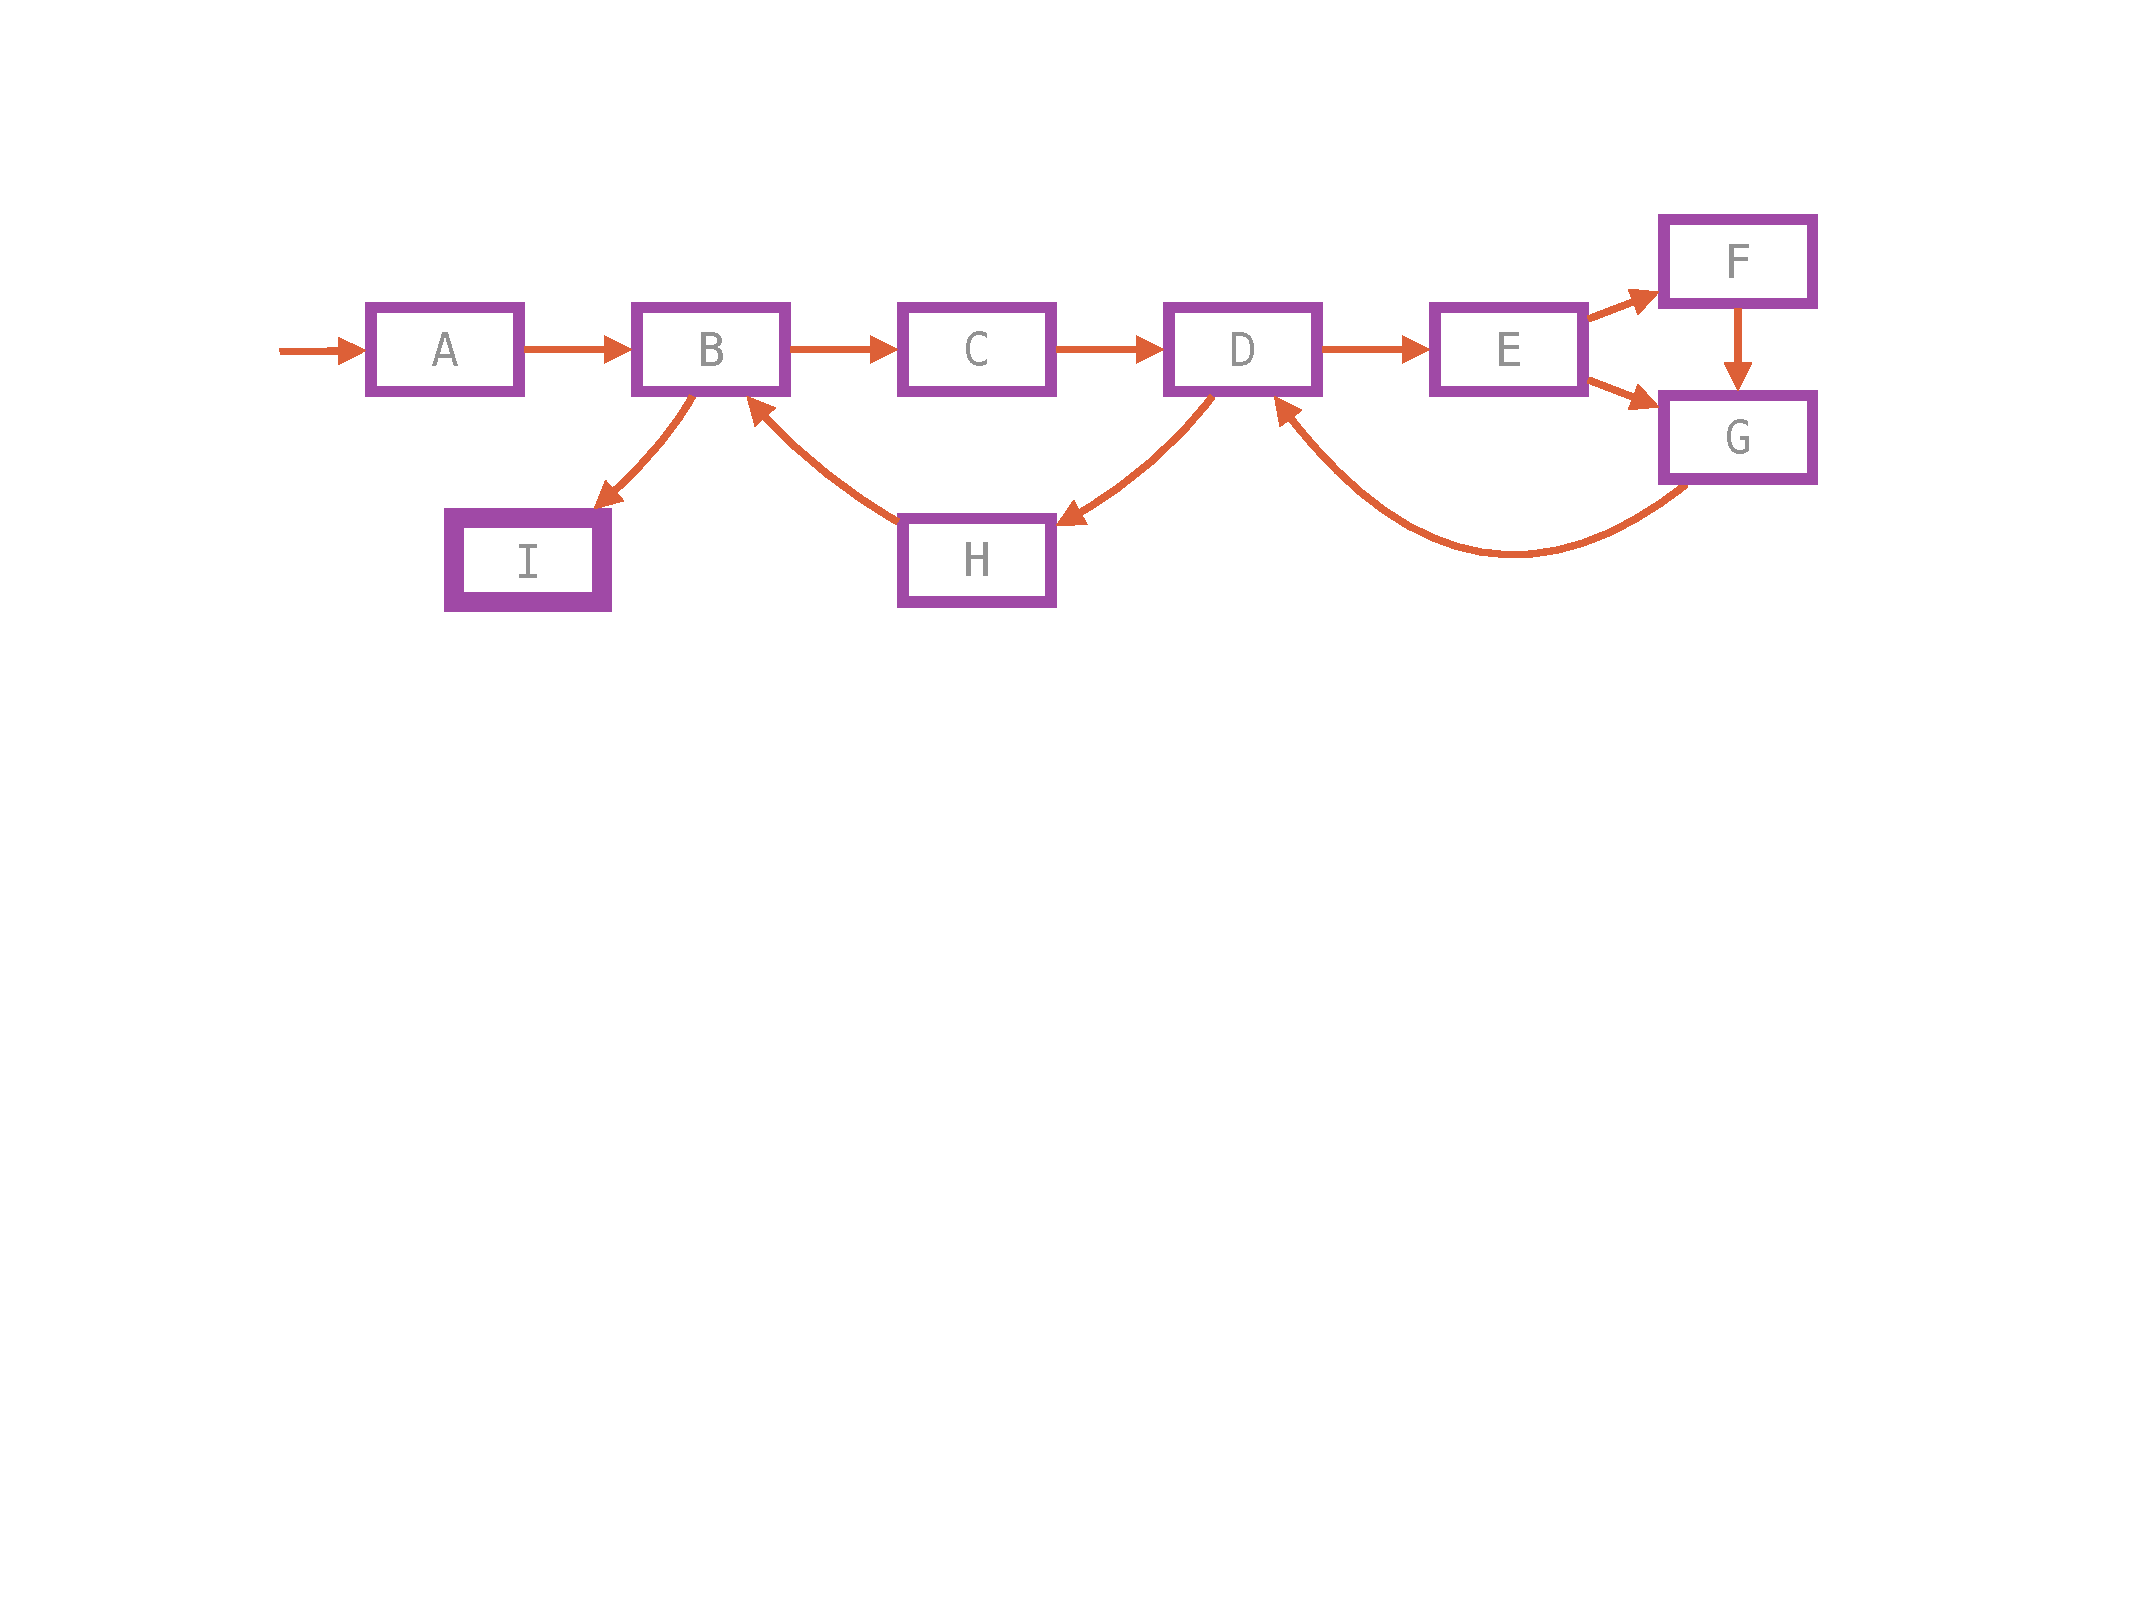
\includegraphics[width=0.8\textwidth]{figs/CFG-2.pdf}

\begin{parts}
\part[8] Provide a simple example of a python function that generates
  this control-flow graph. Unlike the previous question, it should be
  possible for a test set to achieve 100\% node coverage but
  impossible for any test set to satisfy 100\% edge coverage. Do not
  define any auxiliary functions, unless absolutely necessary. Label
  the source code statements with comments corresponding to the CFG
  node names. %
  \boxedanswer{5in}{ %
  }

  \newpage

\part[2] Provide a set of tests that achieve 100\% node coverage.
  \boxedanswer{1.5in}{ %
  FILL IN HERE
}

\part[2] List an infeasible test requirement needed by edge
  coverage.
  \boxedanswer{1.5in}{ %
    FILL IN HERE
  }

  \end{parts}

  \newpage

\question Given the following control flow graph, annotated with
  def-use information:\footnote{Unless otherwise noted, assume
    $def(l) = \emptyset$ and $use(l) = \emptyset$.}

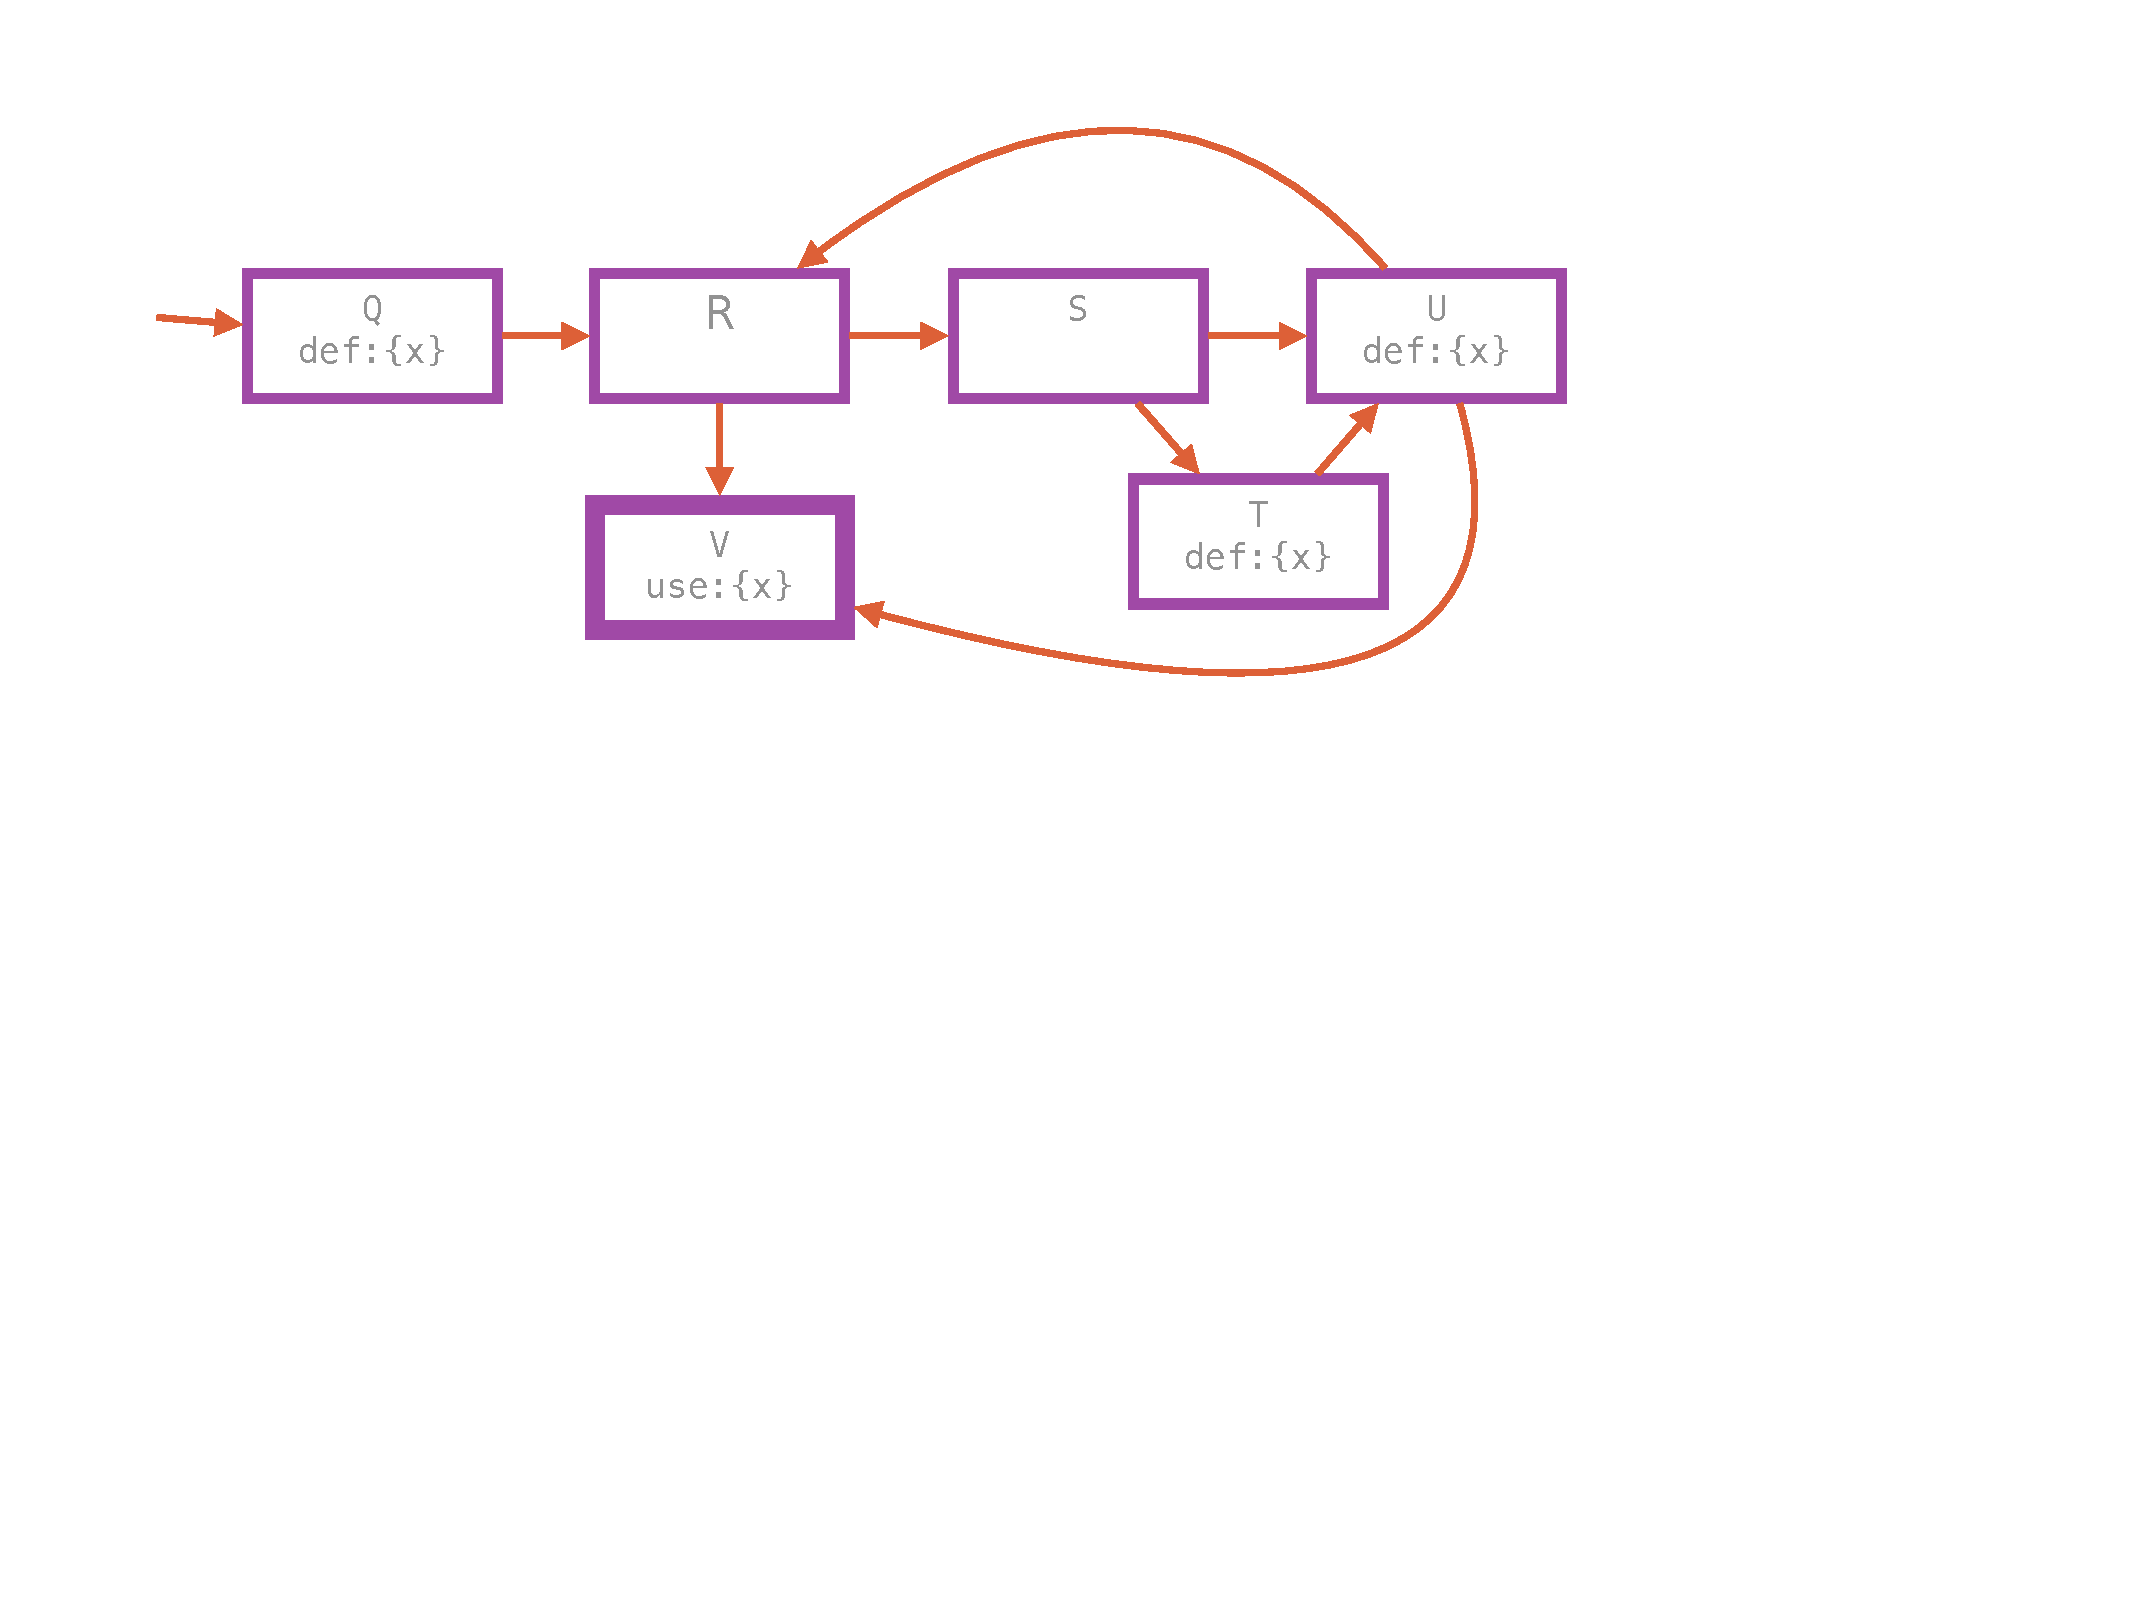
\includegraphics[width=0.8\textwidth]{figs/DU-CFG.pdf}

And the following test paths:
\begin{description}
  \item[TP$_1$:] [Q, R, S, T, U, V]
  \item[TP$_2$:] [Q, R, S, U, V]
  \item[TP$_3$:] [Q, R, S, U, R, V]
  \item[TP$_4$:] [Q, R, V]
  \end{description}

\begin{parts}
\part[5] List all the DU-paths with respect to
  \mintinline{python}{x}. (Note: Include \textbf{all} DU-paths, even
  those that are subpaths of other DU-paths).

Please use the format:

\begin{center}
	du (A, G, \mintinline{python}{y}): [A, B, C, ...]
\end{center}
  \boxedanswer{1.5in}{ %
  du (1, 6, $X$): [1, 2, 6] \\
  du (4, 6, $X$): [ ] \\
  du (5, 6, $X$): [5, 2, 6], [5, 6] \\
}

\part[4] Which DU-paths do each of the TP$_i$ tour?
Please format your answer as
\begin{center}
  TP$_1$ tours \{[A, B, C, ...], …\}
  TP$_2$ tours \{[A, B, C, ...], …\}
\end{center}
\boxedanswer{1.5in}{ %
  T1 tours [5, 6] \\
}

\part[2] List a minimal subset of \{TP$_1$, TP$_2$, TP$_3$, TP$_4$\}
  that satisfies all-defs coverage with respect to \mintinline{python}{x}.
  \boxedanswer{1.5in}{ %
    \{t1, t4\}
    Answer can also be {t2 , t4}
  }

\part[2] List a minimal subset of \{TP$_1$, TP$_2$, TP$_3$, TP$_4$\}
  that satisfies all-uses coverage with respect to \mintinline{python}{x}.
  \boxedanswer{1.5in}{ %
    \{t2,t4\} Answer can
    also be {t1, t4} and {t3, t4} }

\part[3] List a minimal subset of \{TP$_1$, TP$_2$, TP$_3$, TP$_4$\}
  that satisfies all-du-paths coverage with respect to
  \mintinline{python}{x}.%
  \boxedanswer{1.5in}{ %
    % d1 -> u8: t2
    % d1 -> u7: t4
    % d2 -> u8: t1
    % d5 -> u7: t3
    % d5 -> u8: t3
    % \{t1, t2, t3, t4\}

    % OR

    \{t1, t3, t4\}
    or
    \{t2, t3, t4\}
  }
\end{parts}

\question Answer the following questions for the
  \mintinline{python}{checkIt} function shown below.

\begin{minted}{python}
def checkIt(a: bool, b: bool, c: int, d: int) -> None:
    if (a and b) or (c < d):
        print("P is true")
    else:
        if d < c:
            print("P isn't true and c is not equal to d")
        else:
            print("P isn't true and c is equal to d")
\end{minted}

\begin{parts}
\part[3] List all predicates in \mintinline{python}{checkIt}, followed
  by a list of the individual clauses in each predicate.
  Use the format ``predicate1: clause1, clause2, ...''
  \boxedanswer{1.5in}{ %
    $(a \wedge b) \vee (c < d): a, b, c < d$ \\
    $ d < c: d < c$
}

% One point for each in TR
\part[8] Derive a test set satisfying CACC but not RACC for the first
  predicate in \mintinline{python}{checkIt}, and explain why it fails
  RACC. %
  \boxedanswer{5in}{ %
	% The truth table of the predicate in (a) is: \\
	% \begin{tabular}{l|l|l|l|l}
	% 	& a & b & c & P \\ \hline
	% 1 & F & F & F & F \\ \hline
	% 2 & F & F & T & F \\ \hline
	% 3 & F & T & F & F \\ \hline
	% 4 & F & T & T & F \\ \hline
	% 5 & T & F & F & F \\ \hline
	% 6 & T & F & T & T \\ \hline
	% 7 & T & T & F & T \\ \hline
	% 8 & T & T & T & T
	% \end{tabular}
	The following forms of ACC: GACC, CACC, and RACC were accepted as correct answers.

	Make $a$ major then we need $c < d=\bot$ and $b=\top$ for $a$ to determine \(p = (a \wedge b) \vee (c < d)\).
	\[
	TR_a = \{ (a = \top, b = \top, c < d = \bot),\; (a = \bot, b = \top, c < d = \bot)\}
	\]

	Make $b$ major then we need $c=\bot$ and $a=\top$ to determine
	\(p = (a \wedge b) \vee (c < d)\).

	\[
	TR_b = \{ (a = \top, b = \bot, c < d = \bot),\; (a = \top, b = \top, c < d = \bot)\}
	\]

	Make $c$ major then we need $(a \wedge b)=\bot$ to determine
	\(p = (a \wedge b) \vee (c < d)\).

	\[
	TR_{c < d} = \{ (a = \bot, b = \bot, c < d = \bot),\; (a = \bot, b =
        \bot, c < d = \top)\}
	\]

	This gives us

	\[
	TR = TR_a \cup TR_b \cup TR_{c < d} \cup TR_{d < c}
	\]

	\[
	TR = \left\{
	\begin{aligned}
	& (a = \top, b = \top, c < d = \bot),\\
	& (a = \bot, b = \top, c < d = \bot),\\
	& (a = \top, b = \bot, c < d = \bot),\\
	& (a = \bot, b = \bot, c < d = \bot),\\
	& (a = \bot, b = \bot, c < d = \top) \\
        & (d < c = \top) \\
        & (d < c = \bot) \\
      \end{aligned}
    \right\}
  \]
  Final test set:
  \begin{description}
  \item[R1] [a $\mapsto$ true, b $\mapsto$ true, c $\mapsto$ 5, d $\mapsto$ 3]
  \item[R2] [a $\mapsto$ false, b $\mapsto$ true, c $\mapsto$ 5, d $\mapsto$ 3]
  \item[R3] [a $\mapsto$ true, b $\mapsto$ false, c $\mapsto$ 5, d $\mapsto$ 3]
  \item[R4] [a $\mapsto$ false, b $\mapsto$ false, c $\mapsto$ 2, d $\mapsto$ 5]
  \item[R5] [a $\mapsto$ false, b $\mapsto$ false, c $\mapsto$ 5, d $\mapsto$ 2]
  \end{description}
}

\end{parts}

\newpage

\question The function \mintinline{python}{average_in_range()} below
  is intended to return the average (rounded down) of the elements of
  \mintinline{python}{arr} that are strictly positive and strictly
  less than \mintinline{python}{cap}, and to return 0 when there are
  no such elements.

\begin{minted}{python}
def average_in_range(arr, cap):
    total = 0
    count = 0
    i = 0
    while i < len(arr):
        if arr[i] > 0 and arr[i] < cap:
            total = total + arr[i]
            count = count + 1
        i = i + 1
    return total // count
\end{minted}

  Throughout this question, consider the test set
  \begin{description}
    \item[T$_1$:] \mintinline{python}{average_in_range([5, -1, 20], 10)}
    \item[T$_2$:] \mintinline{python}{average_in_range([4, 6], 10)}
    \end{description}
    Note that both of these tests return the expected value, and thus
    pass.

\begin{parts}

\part[3] Draw the control flow graph of
  \mintinline{python}{average_in_range()}, grouping statements into
  basic blocks and labelling each node with the line numbers it
  covers.
  \boxedanswer{5in}{ %
    Six nodes: \texttt{BB2-4} (the three initializations), \texttt{C5}
    (the loop condition), \texttt{C6} (the \texttt{if} condition),
    \texttt{BB7-8} (the two updates), \texttt{BB9}
    (\texttt{i = i + 1}), and \texttt{BB10} (the return).

    Seven edges: \texttt{(BB2-4, C5)}, \texttt{(C5, C6)},
    \texttt{(C5, BB10)}, \texttt{(C6, BB7-8)}, \texttt{(C6, BB9)},
    \texttt{(BB7-8, BB9)}, \texttt{(BB9, C5)}.
  }
\part[1] How many test requirements does node coverage impose?
  \boxedanswer{1in}{ %
    Node coverage imposes 6 requirements.
  }

\part[1] How many does edge coverage impose?
  \boxedanswer{1in}{ %
    Edge coverage imposes 7 requirements.
  }

\part[2] Give the test paths toured by each of the two tests
  above. Taken together, do they achieve 100\% edge coverage? %
  \boxedanswer{2in}{ %
    $t_1$: \texttt{[BB2-4, C5, C6, BB7-8, BB9, C5, C6, BB9, C5, C6,
      BB9, C5, BB10]}

    $t_2$: \texttt{[BB2-4, C5, C6, BB7-8, BB9, C5, C6, BB7-8, BB9, C5,
      BB10]}

    $t_1$ alone tours all seven edges: element 5 takes
    \texttt{(C6, BB7-8)}, elements $-1$ and 20 both take
    \texttt{(C6, BB9)}, and the final loop test takes
    \texttt{(C5, BB10)}. So $T$ achieves 100\% edge coverage (and
    therefore 100\% node coverage).
  }

\part[4] Show that this set of tests satisfies Correlated Active
  Clause Coverage for the predicate on line 6 by identifying which
  required truth assigment each test supplies, noting the major and
  minor clauses in each requirement. %
  \boxedanswer{5in}{ %
    Write $c_1$ for \mintinline{python}{arr[i] > 0} and $c_2$ for
    \mintinline{python}{arr[i] < cap}, so $p = c_1 \wedge c_2$.

    \textbf{$c_1$ major:} $c_1$ determines $p$ when $c_2 = \top$. Need
    $(c_1, c_2) = (\top, \top)$ with $p = \top$ and $(\bot, \top)$
    with $p = \bot$. In $t_1$: element 5 gives $(\top, \top)$; element
    $-1$ gives $(\bot, \top)$, since $-1 < 10$.

    \textbf{$c_2$ major:} $c_2$ determines $p$ when $c_1 = \top$. Need
    $(\top, \top)$ and $(\top, \bot)$. In $t_1$: element 5 gives
    $(\top, \top)$; element 20 gives $(\top, \bot)$.

    All four evaluations occur within $t_1$, so $T$ satisfies CACC.
  }

\part[5] List all du-paths with respect to \mintinline{python}{count}.
  For each one, state whether this test set tours it.
  \boxedanswer{5in}{ %
    \mintinline{python}{count} is defined at \texttt{BB2-4} and at
    \texttt{BB7-8}, and used at \texttt{BB7-8} and \texttt{BB10}. Four
    du-paths:

    \begin{tabular}{llc}
      \textbf{du-pair} & \textbf{du-path} & \textbf{toured by $T$?} \\
      \hline
      (BB2-4, BB7-8) & [BB2-4, C5, C6, BB7-8] & yes ($t_1$, $t_2$) \\
      (BB2-4, BB10) & [BB2-4, C5, BB10] & \textbf{no} \\
      (BB7-8, BB7-8) & [BB7-8, BB9, C5, C6, BB7-8] & yes ($t_2$) \\
      (BB7-8, BB10) & [BB7-8, BB9, C5, BB10] & yes ($t_2$) \\
    \end{tabular}

    The second one is untoured because both tests enter the loop body
    at least once, so neither goes straight from \texttt{C5} to
    \texttt{BB10}.
  }

\part[2] Does this test set satisfy all-defs coverage with respect to
  \mintinline{python}{count}? Does it satisfy all-uses coverage?
  Justify both answers in one to two sentences.  %
  \boxedanswer{4in}{ %
    \textbf{All-defs: yes.} Each def needs only one du-path toured.
    The def at \texttt{BB2-4} is covered by \texttt{[BB2-4, C5, C6,
      BB7-8]}, and the def at \texttt{BB7-8} by \texttt{[BB7-8, BB9,
      C5, BB10]}.

    \textbf{All-uses: no.} Every (def, use) pair needs its own
    du-path, and the pair (\texttt{BB2-4}, \texttt{BB10}) is not
    toured by either test.
  }

\part[3] Neither test induces a failure, but
  \mintinline{python}{average_in_range()} nevertheless contains a
  fault. Give a test input that reveals it, and explain why satisfying
  all-uses coverage with respect to \mintinline{python}{count} would
  have forced such a test. %
  \boxedanswer{4in}{ %
    The function never guards against \mintinline{python}{count == 0},
    so line 10 divides by zero.
    \mintinline{python}{average_in_range([], 10)} raises
    \texttt{ZeroDivisionError} where the specification requires 0.

    Touring \texttt{[BB2-4, C5, BB10]} means leaving the loop without
    ever entering the body, which is only possible when
    \mintinline{python}{arr} is empty --- and that is exactly the case
    in which \mintinline{python}{count} is still 0 at line 10.

    (Edge-pair coverage would also force it, since
    \texttt{[BB2-4, C5, BB10]} is a path of length 2. Note also that
    \mintinline{python}{average_in_range([-1], 10)} fails for the same
    reason, but no criterion in this question requires it.)
  }

\part[3] In one or two sentences, what does this example show about the
  relationship between a test suite's coverage and its ability to
  detect faults?
  \boxedanswer{2.5in}{ %
    Satisfying a criterion guarantees only that certain paths are
    executed, not that a fault is exposed --- $T$ reaches every node,
    every edge, and every clause-determining evaluation, and still
    misses the fault. Stronger criteria shrink the gap but never close
    it, and no criterion says anything about whether the oracle
    actually checks the right thing.
  }

\end{parts}

\end{questions}

\end{document}
